\documentclass[compress]{beamer}
\usepackage{irbookslide}
\usepackage{irilmenau2}
\usepackage{tikz}
\usepackage{url}
\usepackage{ifxetex}
%\RequireXeTeX
\usepackage{fontspec} % zahteva paket euenc
\usepackage{xunicode}
\usepackage{xltxtra}
\usepackage{polyglossia}
\usepackage{minted}
\usepackage{algorithmic}
\renewcommand{\algorithmicrequire}{\textbf{Input:}}
\renewcommand{\algorithmicensure}{\textbf{Output:}}
\usepackage{xcolor,colortbl}
\usepackage{textcomp}
%\setdefaultlanguage[script=Latin]{serbian}

\title{Mape, heš tabele, skip liste, skupovi}
\author{\textcopyright \ \ Goodrich, Tamassia, Goldwasser}
\institute{Katedra za informatiku, Fakultet tehničkih nauka, Univerzitet u
Novom Sadu}
\date{2014.}
\subject{Predavanja sa ASP}

\begin{document}

\frame{\titlepage}

\section[Mapa]{Pojam mape}
\begin{frame}[fragile]
  \frametitle{Mapa}
  \begin{itemize}
    \item Pythonov rečnik (klasa \textbf{dict}) preslikava \textbf{ključeve} na \textbf{vrednosti} 
    \item drugo ime: \myred{asocijativni niz} ili \myred{mapa}
    \item ključevi su jedinstveni (nema ponavljanja)
    \item vrednosti ne moraju biti jedinstvene
  \end{itemize}
  \begin{center}
    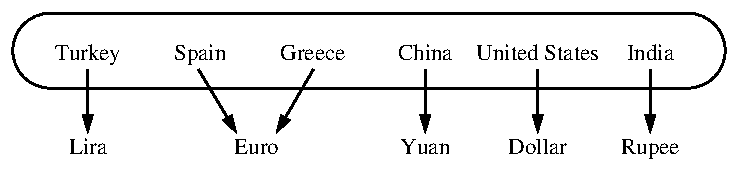
\includegraphics[width=10cm]{asp-10-pic01.pdf}
  \end{center}
\end{frame}

\begin{frame}[fragile]
  \frametitle{Mapa ATP: osnovne operacije}
  \begin{center}
    \begin{tabular}{rp{8cm}}
      \textbf{\texttt{M[k]}} & vraća vrednost $v$ vezanu za ključ $k$ u mapi $M$; ako ne postoji, izaziva \texttt{KeyError}; implementira je \texttt{\_\_getitem\_\_} \\ \hline
      \textbf{\texttt{M[k] = v}} & dodeljuje vrednost $v$ ključu $k$ u mapi $M$; ako ključ već postoji, zamenjuje staru vrednost; implementira je \texttt{\_\_setitem\_\_} \\ \hline
      \textbf{\texttt{del M[k]}} & uklanja element sa ključem $k$ iz mape $M$; ako ne postoji, izaziva \texttt{KeyError}; implementira je \texttt{\_delitem\_\_} \\ \hline
      \textbf{\texttt{len(M)}} & vraća broj elemenata u mapi $M$; implementira je \texttt{\_\_len\_\_} \\ \hline
      \textbf{\texttt{iter(M)}} & generiše listu \textbf{ključeva} iz mape $M$;  implementira je \texttt{\_\_iter\_\_} \\
    \end{tabular}
  \end{center}
\end{frame}

\begin{frame}[fragile]
  \frametitle{Mapa ATP: dodatne operacije}
  \begin{center}
    \begin{tabular}{rp{6cm}}
      \textbf{\texttt{k in M}} & vraća \texttt{True} ako mapa $M$ sadrži ključ $k$; implementira je \texttt{\_\_contains\_\_} \\ \hline
      \textbf{\texttt{M.get(k, d=None)}} & vraća $M[k]$ ako ključ $k$ postoji u $M$; inače vraća default vrednost $d$; ne izaziva \texttt{KeyError} \\ \hline
      \textbf{\texttt{M.setdefault(k, d)}} & ako $k$ postoji u mapi, vraća $M[k]$; ako ne postoji, postavlja $M[k]=d$ i vraća $d$ \\ \hline
      \textbf{\texttt{M.pop(k, d=None)}} & uklanja element sa ključem $k$ i vraća vezanu vrednost $v$; ako ključ $k$ nije u mapi $M$, vraća $d$ ili izaziva \texttt{KeyError} ako je $d$ jednako \texttt{None}
    \end{tabular}
  \end{center}
\end{frame}

\begin{frame}[fragile]
  \frametitle{Mapa ATP: još malo operacija}
  \begin{center}
    \begin{tabular}{rp{8cm}}
      \textbf{\texttt{M.popitem()}} & uklanja neki element mape i vraća ($k$,$v$); ako je mapa prazna izaziva \texttt{KeyError} \\ \hline
      \textbf{\texttt{M.clear()}} & uklanja sve elemente iz mape \\ \hline
      \textbf{\texttt{M.keys()}} & vraća skup svih ključeva iz $M$ \\ \hline
      \textbf{\texttt{M.values()}} & vraća skup svih vrednosti iz $M$ \\ \hline
      \textbf{\texttt{M.items()}} & vraća skup svih parova ($k$,$v$) iz $M$ \\ \hline
      \textbf{\texttt{M.update(M2)}} & dodeljuje \texttt{M[k]=v} za svaki ($k$,$v$) iz $M2$ \\ \hline
      \textbf{\texttt{M == M2}} & vraća \texttt{True} ako mape sadrže iste parove ($k$,$v$) \\ \hline
      \textbf{\texttt{M != M2}} & vraća \texttt{True} ako mape ne sadrže iste parove ($k$,$v$)
    \end{tabular}
  \end{center}
\end{frame}

\begin{frame}[fragile,shrink]
  \frametitle{Mapa ATP: primer}
  \begin{center}
    \begin{tabular}{lcl}
      \textbf{operacija} & \textbf{rezultat} & \textbf{mapa} \\ \hline
      \texttt{len(M)} & 0 & \texttt{\{ \}} \\
      \texttt{M['K']=2} & -- & \texttt{\{'K':2\}} \\
      \texttt{M['B']=4} & -- & \texttt{\{'K':2, 'B':4\}} \\
      \texttt{M['U']=2} & -- & \texttt{\{'K':2, 'B':4, 'U':2\}} \\
      \texttt{M['V']=8} & -- & \texttt{\{'K':2, 'B':4, 'U':2, 'V':8\}} \\
      \texttt{M['K']=9} & -- & \texttt{\{'K':9, 'B':4, 'U':2, 'V':8\}} \\
      \texttt{M['B']} & 4 & \texttt{\{'K':9, 'B':4, 'U':2, 'V':8\}} \\
      \texttt{M['X']} & \texttt{KeyError} & \texttt{\{'K':9, 'B':4, 'U':2, 'V':8\}} \\
      \texttt{M.get('F')} & \texttt{None} & \texttt{\{'K':9, 'B':4, 'U':2, 'V':8\}} \\
      \texttt{M.get('F', 5)} & \texttt{5} & \texttt{\{'K':9, 'B':4, 'U':2, 'V':8\}} \\
      \texttt{M.get('K', 5)} & \texttt{9} & \texttt{\{'K':9, 'B':4, 'U':2, 'V':8\}} \\
      \texttt{len(M)} & \texttt{4} & \texttt{\{'K':9, 'B':4, 'U':2, 'V':8\}} \\
      \texttt{del M['V']} & -- & \texttt{\{'K':9, 'B':4, 'U':2\}} \\
      \texttt{M.pop('K')} & 9 & \texttt{\{'B':4, 'U':2\}} \\
      \texttt{M.keys()} & \texttt{'B','U'} & \texttt{\{'B':4, 'U':2\}} \\
      \texttt{M.values()} & \texttt{4,2} & \texttt{\{'B':4, 'U':2\}} \\
      \texttt{M.items()} & \texttt{('B',4),('U',2)} & \texttt{\{'B':4, 'U':2\}} \\
      \texttt{M.setdefault('B',1)} & \texttt{4} & \texttt{\{'B':4, 'U':2\}} \\
      \texttt{M.setdefault('A',1)} & \texttt{1} & \texttt{\{'A':1, 'B':4, 'U':2\}} \\
      \texttt{M.popitem()} & \texttt{('B',4)} & \texttt{\{'A':1, 'U':2\}}
    \end{tabular}
  \end{center}
\end{frame}

\begin{frame}[fragile]
  \frametitle{Različite implementacije mape}
  \begin{center}
    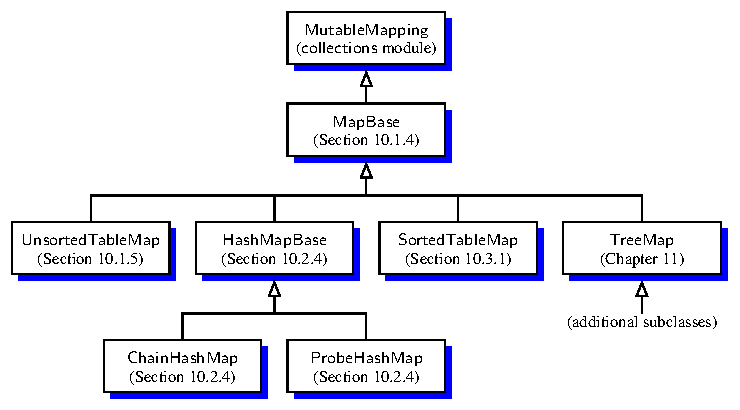
\includegraphics[width=11cm]{asp-10-pic02.pdf}
  \end{center}
\end{frame}

\begin{frame}[fragile,shrink]
  \frametitle{Implementacija MapBase}
\begin{minted}[linenos=false]{python}
from collections import MutableMapping

class MapBase(MutableMapping):
  """Our own abstract base class that includes a nonpublic _Item class."""

  #-- nested _Item class --
  class _Item:
    """Lightweight composite to store key-value pairs as map items."""
    __slots__ = '_key', '_value'

    def __init__(self, k, v):
      self._key = k
      self._value = v

    def __eq__(self, other):               
      return self._key == other._key   # compare items based on their keys

    def __ne__(self, other):
      return not (self == other)       # opposite of __eq__

    def __lt__(self, other):               
      return self._key < other._key    # compare items based on their keys
\end{minted}
\end{frame}

\begin{frame}[fragile]
  \frametitle{Mapa pomoću liste}
  \begin{itemize}
    \item jedna moguća implementacija mape je pomoću dvostruko spregnute liste 
    \item elemente čuvamo u proizvoljnom redosledu
  \end{itemize}
  \begin{center}
    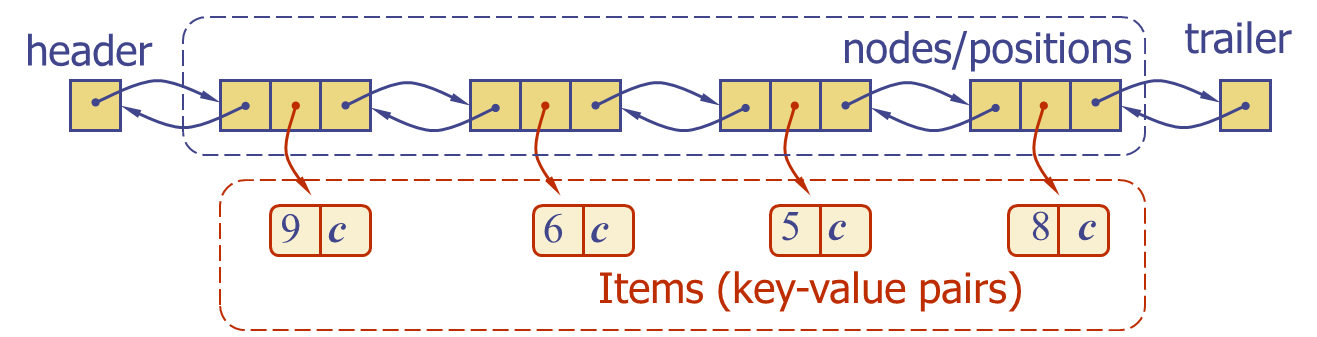
\includegraphics[width=10cm]{asp-10-pic03.png}
  \end{center}
\end{frame}

\begin{frame}[fragile,shrink]
  \frametitle{Mapa pomoću liste: implementacija $_1$}
\begin{minted}[linenos=false]{python}
class UnsortedTableMap(MapBase):
  """Map implementation using an unordered list."""

  def __init__(self):
    """Create an empty map."""
    self._table = []                              # list of _Item's
  
  def __getitem__(self, k):
    """Return value associated with key k (raise KeyError if not found)."""
    for item in self._table:
      if k == item._key:
        return item._value
    raise KeyError('Key Error: ' + repr(k))

  def __setitem__(self, k, v):
    """Assign value v to key k, overwriting existing value if present."""
    for item in self._table:
      if k == item._key:                          # Found a match:
        item._value = v                           # reassign value
        return                                    # and quit    
    # did not find match for key
    self._table.append(self._Item(k,v))
\end{minted}
\end{frame}

\begin{frame}[fragile,shrink=25]
  \frametitle{Mapa pomoću liste: implementacija $_2$}
\begin{minted}[linenos=false]{python}
  def __delitem__(self, k):
    """Remove item associated with key k (raise KeyError if not found)."""
    for j in range(len(self._table)):
      if k == self._table[j]._key:                # Found a match:
        self._table.pop(j)                        # remove item
        return                                    # and quit    
    raise KeyError('Key Error: ' + repr(k))

  def __len__(self):
    """Return number of items in the map."""
    return len(self._table)

  def __iter__(self):                             
    """Generate iteration of the map's keys."""
    for item in self._table:
      yield item._key                             # yield the KEY
\end{minted}
\end{frame}

\begin{frame}[fragile]
  \frametitle{Mapa pomoću liste: performanse}
  \begin{itemize}
    \item \textbf{dodavanje} traje $O(1)$ -- novi element možemo dodati na početak ili na kraj  
    \item \textbf{traženje} ili \textbf{uklanjanje} traje $O(n)$ -- u najgorem slučaju (nije pronađen element) mora se proći kroz celu listu
    \item ovakva implementacija je korisna samo za mape sa malim brojem elemenata
    \item ili ako je dodavanje najčešća operacija, dok se traženje i uklanjanje retko obavljaju
  \end{itemize}
\end{frame}

\section[Hash tabela]{Hash tabela}
\begin{frame}[fragile]
  \frametitle{Hash tabela}
  \begin{itemize}
    \item mapa omogućava pristup korišćenjem \textbf{ključeva} kao \textbf{indeksa} -- \texttt{M[k]}  
    \item zamislimo mapu koja kao ključeve korisiti cele brojeve iz intervala $[0, N-1]$ za neko $N > n$
    \item za čuvanje elemenata možemo koristiti \myred{lookup} niz dužine $N$
    \item npr. mapa sa elementima $(1,D), (3,Z), (6,C), (7,Q)$
  \end{itemize}
  \begin{center}
    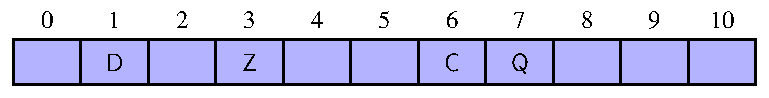
\includegraphics[width=10cm]{asp-10-pic04.pdf}
  \end{center}
  \begin{itemize}
    \item operacije su $O(1)$  
  \end{itemize}
\end{frame}

\begin{frame}[fragile]
  \frametitle{Hash tabela}
  \begin{itemize}
    \item šta ako je $N >> n$ ?  
    \item šta ako ključevi nisu celi brojevi?
    \item pretvorićemo ključeve u cele brojeve pomoću \myred{hash funkcije}
    \item dobra hash funkcija će ravnomerno distribuirati ključeve u $[0,N-1]$
    \item ali može biti duplikata
    \item duplikate ćemo čuvati u ,,kantama`` -- tzv. \myred{bucket array}
  \end{itemize}
  \begin{center}
    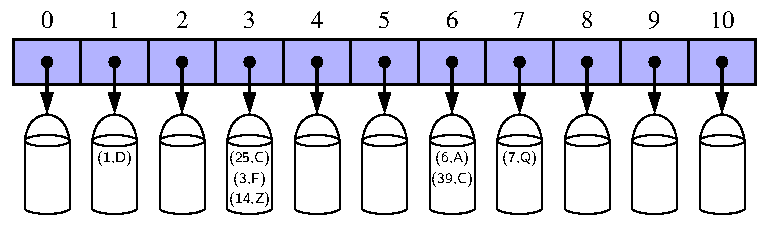
\includegraphics[width=10cm]{asp-10-pic05.pdf}
  \end{center}
\end{frame}

\begin{frame}[fragile]
  \frametitle{Hash tabela}
  \begin{itemize}
    \item šta ako je $N >> n$ ?  
    \item šta ako ključevi nisu celi brojevi?
    \item pretvorićemo ključeve u cele brojeve pomoću \myred{hash funkcije}
    \item dobra hash funkcija će ravnomerno distribuirati ključeve u $[0,N-1]$
    \item ali može biti duplikata
    \item duplikate ćemo čuvati u ,,kantama`` -- tzv. \myred{bucket array}
  \end{itemize}
  \begin{center}
    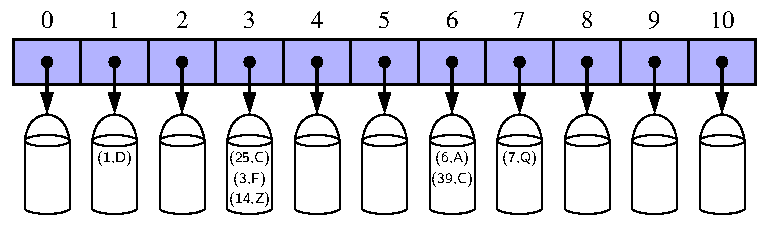
\includegraphics[width=10cm]{asp-10-pic05.pdf}
  \end{center}
\end{frame}

\begin{frame}[fragile]
  \frametitle{Hash funkcija}
  \begin{itemize}
    \item \textbf{hash funkcija} mapira ključeve na indekse u hash tabeli  
    \item npr. poslednje četiri cifre broja telefona
  \end{itemize}
  \begin{center}
    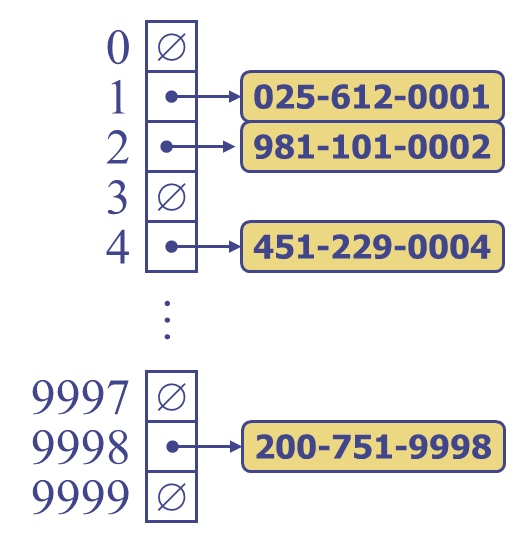
\includegraphics[width=4cm]{asp-10-pic06.png}
  \end{center}
\end{frame}

\begin{frame}[fragile]
  \frametitle{Hash funkcija}
  \begin{itemize}
    \item \textbf{hash funkcija} mapira ključ $k$ na ceo broj u intervalu $[0,N-1]$
    \item gde je $N$ kapacitet niza kanti $A$
    \item element $(k,v)$ čuvamo u nizu kao $A[h(k)]$
    \item \myred{kolizija}: dve vrednosti ključa koje daju isti hash
    \item dobre hash funkcije imaju \textbf{vrlo malo} kolizija
  \end{itemize}
\end{frame}

\begin{frame}[fragile]
  \frametitle{Hash funkcija}
  \begin{itemize}
    \item često se hash funkcija može posmatrati kao kompozicija dve funkcije:
    \item \myred{hash code}: mapira ključ na ceo broj
    \item \myred{compression function}: mapira hash kôd na broj u intervalu $[0,N-1]$ 
  \end{itemize}
  \begin{center}
    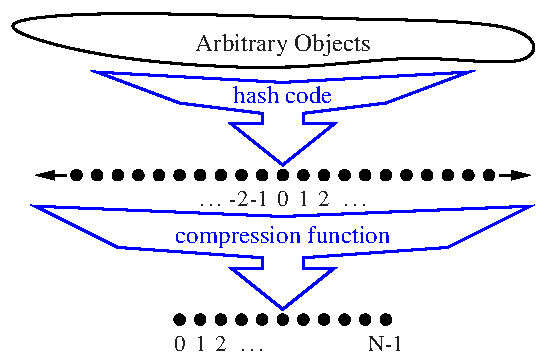
\includegraphics[width=7cm]{asp-10-pic07.pdf}
  \end{center}
\end{frame}

\begin{frame}[fragile]
  \frametitle{Hash funkcija}
  \begin{itemize}
    \item ako se hash funkcija posmatra kao \\ \myred{hash code} $\circ$ \myred{compression function}
    \item tada hash code ne zavisi od veličine niza kanti \\ \ \\
    \item vrednosti koje su ,,blizu`` u skupu ključeva ne moraju imati hasheve koji su ,,blizu`` 
  \end{itemize}
\end{frame}

\begin{frame}[fragile]
  \frametitle{Hash code $_1$}
  \begin{itemize}
    \item memorijska adresa
    \begin{itemize}
      \item adresa Python objekta u memoriji kao hash code
      \item dobro osim za numeričke tipove i stringove
    \end{itemize}
    \item integer cast 
    \begin{itemize}
      \item za svaki tip podataka koji se predstavlja sa najviše onoliko bita koliko i \textbf{int} možemo uzeti int interpretaciju njegovih bita
      \item za tipove koji zauzimaju više memorije moramo nekako ,,sažeti`` njegove bite
      \item npr. \textbf{float} broj u Pythonu zauzima 64 bita a hash kod 32; možemo izabrati
      \begin{itemize}
        \item gornjih 32 bita
        \item donjih 32 bita
        \item neku kombinaciju sva 64 bita: XOR ili zbir gornje i donje polovine, itd.
      \end{itemize}
    \end{itemize}
  \end{itemize}
\end{frame}

\begin{frame}[fragile]
  \frametitle{Hash code $_2$}
  \begin{itemize}
    \item suma komponenti
    \begin{itemize}
      \item adresa Python objekta u memoriji kao hash code
      \item dobro osim za numeričke tipove i stringove
    \end{itemize}
    \item integer cast 
    \begin{itemize}
      \item za svaki tip podataka koji se predstavlja sa najviše onoliko bita koliko i \textbf{int} možemo uzeti int interpretaciju njegovih bita
      \item za tipove koji zauzimaju više memorije moramo nekako ,,sažeti`` njegove bite
      \item npr. \textbf{float} broj u Pythonu zauzima 64 bita a hash kod 32; možemo izabrati
      \begin{itemize}
        \item gornjih 32 bita
        \item donjih 32 bita
        \item neku kombinaciju sva 64 bita: XOR ili zbir gornje i donje polovine, itd.
      \end{itemize}
    \end{itemize}
  \end{itemize}
\end{frame}

\end{document}